% tikzpic.tex
\documentclass[crop,tikz]{standalone}% 'crop' is the default for v1.0, before it was 'preview'
%\usetikzlibrary{...}% tikz package already loaded by 'tikz' option
\usepackage{amsmath,amsthm,amssymb,mathrsfs,amsfonts,dsfont}
\usetikzlibrary{plotmarks}
\usepackage{pgfplots}
\usepgfplotslibrary{fillbetween}

\begin{document}

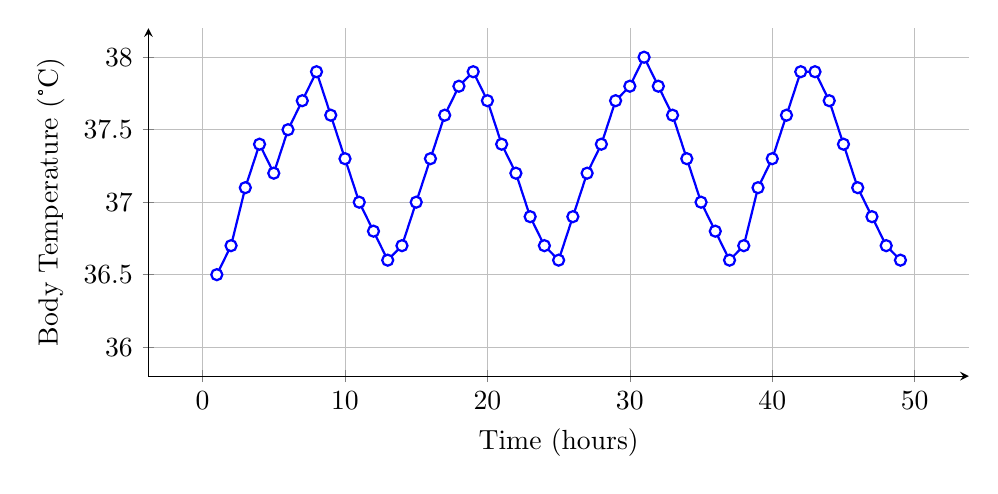
\begin{tikzpicture}
    \begin{axis}[
        width=12cm, height=6cm,
        xlabel={Time (hours)},
        ylabel={Body Temperature (°C)},
        grid=both,
        grid style={line width=.1pt, draw=gray!10},
        major grid style={line width=.2pt,draw=gray!50},
        axis lines=left,
        enlargelimits=true,
        ymin=36, ymax=38,
        xtick={0,10,20,30,40,50},
        ytick={36, 36.5, 37, 37.5, 38},
        scatter,
        mark=*,
        mark size=2pt,
        scatter/classes={
            a={mark=*,fill=white}
        }
    ]
        % Combine scatter and line plot
        \addplot[blue, thick, scatter, scatter src=explicit symbolic] table[x index=0, y index=1, meta index=2] {
            0   36.7   a
            1   36.5   a
            2   36.7   a
            3   37.1   a
            4   37.4   a
            5   37.2   a
            6   37.5   a
            7   37.7   a
            8   37.9   a
            9   37.6   a
            10  37.3   a
            11  37.0   a
            12  36.8   a
            13  36.6   a
            14  36.7   a
            15  37.0   a
            16  37.3   a
            17  37.6   a
            18  37.8   a
            19  37.9   a
            20  37.7   a
            21  37.4   a
            22  37.2   a
            23  36.9   a
            24  36.7   a
            25  36.6   a
            26  36.9   a
            27  37.2   a
            28  37.4   a
            29  37.7   a
            30  37.8   a
            31  38.0   a
            32  37.8   a
            33  37.6   a
            34  37.3   a
            35  37.0   a
            36  36.8   a
            37  36.6   a
            38  36.7   a
            39  37.1   a
            40  37.3   a
            41  37.6   a
            42  37.9   a
            43  37.9   a
            44  37.7   a
            45  37.4   a
            46  37.1   a
            47  36.9   a
            48  36.7   a
            49  36.6   a
        };
    \end{axis}
\end{tikzpicture}

\end{document}